documentclass[tikz,12pt]{standalone}


\begin{document}
\begin{tikzpicture}

%主线轴
\draw [](0,0) -- (100,0);

\draw (-3,-4) rectangle (103,0);

%细小刻度
\foreach \x in {1,2,...,99}
  \draw [](\x,0) -- (\x,-1) ;

%5分之一刻度
\foreach \y in {0,5,...,100}
  \draw [] (\y,-1.6) -- (\y,0);


%10分之一刻度
\foreach \i in {0,10,...,100}
  \draw [] (\i,-2.2) -- (\i,0)
  node[below=2.5cm] {\Huge \pgfmathprint{int(\i/10)}};

%unit
\node at (101.5,-3) {\Huge  cm};




\end{tikzpicture}
\end{document}
